\begin{frame}
    \frametitle{Fast p2o Map Applications}
    \begin{itemize}
        \item Regardless of the method used to carry out the inversion, there is a need for fast Hessian applications
        \item Most expensive part of Hessian application is the p2o operator (usually applied via forward/adjoint PDE solves)
        \item \emph{Autonomous Dynamical System:} evolution does not depend explicitly on independent variable (e.g. time)
        \begin{itemize}
            \item Here: the mapping \(m(x,t+\tau) \mapsto d(x,t+\tau)\) is the same as the mapping \(m(x,t) \mapsto d(x,t)\)
        \end{itemize}
        \item Exploit (time) \emph{shift invariance} of autonomous dynamical systems
        \begin{itemize}
            \item Reduce computation and storage costs
        \end{itemize}
    \end{itemize}
\end{frame}

\begin{frame}
    \frametitle{Block-Triangular Toeplitz Structure}
    \begin{itemize}
        \item Consider linear time-invariant (LTI) system:
        \[
        \begin{aligned}
        \frac{\partial u}{\partial t} &= \mathcal{A} u + \mathcal{C} m \quad (+\text{BCs}) && \text{in } \Omega \times (0,T), \\
        u &= u_0 && \text{in } \Omega \times \{ 0 \}, \\
        d &= \mathcal{B} u && \text{in } \Omega \times (0,T)
        \end{aligned}
        \]
        \item Discretize (FE + explicit time-stepping):
        \[
        \begin{aligned}
        u_1 &= A u_0 + C m_0 , \\
        u_2 &= A u_1 + C m_1 , \\
        &= A (A u_0 + C m_0) + C m_1 = A^2 u_0 + A^1 C m_0 + A^0 C m_1 , \\
        \vdots \\
        u_{k+1} &= A^{k+1} u_0 + \sum_{i=0}^k A^i C m_{k-i} , \\
        d_{k+1} &= B u_{k+1}
        \end{aligned}
        \]
    \end{itemize}
\end{frame}

\begin{frame}
    \frametitle{Block-Triangular Toeplitz Structure}
    \[
    \begin{aligned}
    \begin{bmatrix}
    d_1 \\
    d_2 \\
    \vdots \\
    d_{k+1} \\
    \vdots \\
    d_{N_t}
    \end{bmatrix}
    &=
    \begin{bmatrix}
    B A^0 C \\
    B A^1 C & B A^0 C \\
    \vdots & \vdots & \ddots \\
    B A^k C & B A^{k-1} C & \cdots & B A^0 C \\
    \vdots & \vdots & & \vdots & \ddots \\
    B A^{N_t-1} C & B A^{N_t-2} C & \cdots & B A^{N_t-(k+1)} C & \cdots & B A^0 C
    \end{bmatrix}
    \begin{bmatrix}
    m_0 \\
    m_1 \\
    \vdots \\
    m_k \\
    \vdots \\
    m_{N_t-1}
    \end{bmatrix}
    \end{aligned}
    \]
    \[
    \begin{aligned}
    \begin{bmatrix}
    d_1 \\
    d_2 \\
    d_3 \\
    \vdots \\
    d_{N_t}
    \end{bmatrix}
    &=
    \begin{bmatrix}
    F_{11} & 0 & 0 & \cdots & 0 \\
    F_{21} & F_{11} & 0 & \cdots & 0 \\
    F_{31} & F_{21} & F_{11} & \ddots & \vdots \\
    \vdots & \vdots & \ddots & \ddots & 0 \\
    F_{N_t,1} & F_{N_t-1,1} & \cdots & F_{21} & F_{11}
    \end{bmatrix}
    \begin{bmatrix}
    m_0 \\
    m_1 \\
    m_2 \\
    \vdots \\
    m_{N_t-1}
    \end{bmatrix}
    \end{aligned}
    \]
    \begin{figure}
        \caption{Defining \(F_{ij} := B A^{i-j} C\), \(i,j=1,2,\ldots,N_t, i \ge j\) and assuming \(u_0=0\) WLOG}
    \end{figure}
\end{frame}

\begin{frame}
    \frametitle{Fast p2o Map Applications}
    \begin{itemize}
        \item shift-invariance \(\Rightarrow\) \(\mathbf{F}\) is \emph{block lower-triangular Toeplitz}
    \end{itemize}
    \begin{figure}
        \includegraphics[width=\textwidth]{animation/block_toeplitz_anim.png}
    \end{figure}
    \begin{itemize}
        \item Only \textbf{one} block row of \(\mathbf{F}^*\) needs to be computed/stored
        \item \(\mathcal{O}(N_dN_mN_t)\) storage vs. \(\mathcal{O}(N_dN_mN_t^2)\) (0.8 TB vs. 800 TB for CSZ)
        \item \(N_d\) adjoint PDE solves instead of \(N_dN_t\)
        \begin{itemize}
            \item Adjoint PDE solved backwards in time with "source" at each observation point
        \end{itemize}
    \end{itemize}
\end{frame}

\begin{frame}
    \frametitle{Distributed Matvec Algorithm: Summary}
    \begin{itemize}
        \item \emph{FFT} of input vector: \(O(N_mN_t\log N_t)\)
        \item \emph{Matvec} in Fourier space: \(O(N_dN_mN_t)\)
        \item \emph{IFFT} of output vector: \(O(N_dN_t\log N_t)\)
        \item Same algorithm for \(\mathbf{F}^*\)
        \begin{itemize}
            \item Broadcast across processor rows and reduce up processor columns
            \item Conjugate transpose SBGEMV
            \item \textbf{No extra storage or communication needed}
        \end{itemize}
        \item Overall cost: \(O(N_dN_mN_t + (N_m+N_d)N_t\log N_t)\) (for single GPU)
        \item Parallel complexity derivation is more involved and left to paper\footnote{\href{https://arxiv.org/pdf/2407.13066}{Fast and Scalable FFT-Based GPU-Accelerated Algorithms for Hessian Actions}}
        \item Algorithm is \emph{exact} and provides \textbf{\(\mathcal{O}(10^4)\) speedups} over PDE solve method for p2o applications
        \item Open-source implementation on \href{https://github.com/s769/FFTMatvec}{GitHub}
    \end{itemize}
\end{frame}

\begin{frame}
    \frametitle{Distributed Matvec Performance}
    \begin{columns}
        \column{0.5\textwidth}
        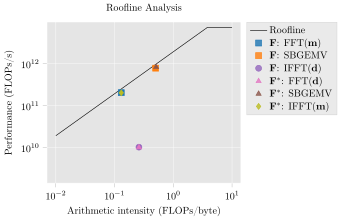
\includegraphics[width=\textwidth]{JMM/images/matvec/roofline.svg}
        \column{0.5\textwidth}
        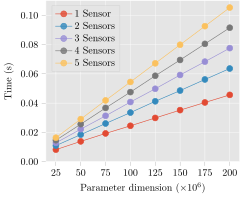
\includegraphics[width=\textwidth]{JMM/images/matvec/single_gpu_scaling.svg}
    \end{columns}
    \begin{figure}
        \caption{Left: Roofline analysis of major kernels (memory-bound); Right: Single GPU p2o matvec times}
    \end{figure}
    \begin{itemize}
        \item Using 4,096 GPUs on \href{https://docs.nersc.gov/systems/perlmutter/architecture/}{\emph{Perlmutter}}, a matvec with \(N_mN_t \sim 1.6\times 10^{11}, N_dN_t\sim2.5\times10^4\) is computed in ~0.2 s
    \end{itemize}
\end{frame}
